\documentclass{article}
\usepackage{geometry}[margin=2cm]
\usepackage{graphicx}

\title{Snake}
\author{Alessandra Sasanelli, Simone Maccario}
\date{\today}

\begin{document}
	\maketitle
	\abstract{
		In this document we would like to discuss our proposal for the PF1 project.
		We decided to reproduce the "Snake" game; here we will explain our intentions 
		and ideas for implementing this game in the racket ASL language.
	}
	
	\section{The game}
	Our aim for this project is to recreate the Snake game.
	This game consists of 3 basic elements, which are a snake, an apple and the background: on the background, the snake moves at specified pace whilst the apple is positioned at available random positions at the starting of the game or if the apple has been eaten.
	The objective of the game is to get your snake eat as many apples as it can to become bigger. The user looses the game if the snake hits the border or it hits itself.
	To interact with the application, the user can use the keyboards' buttons arrow "up", "down", "left", "right", the "r" button and the "escape" button. 
	The firsts four buttons are needed to change the direction of the snake; the "r" button is, instead, needed to start a new game if you lost the previous game; the escape button is needed to quit the application.
	\begin{figure}[h!]
		\centering
		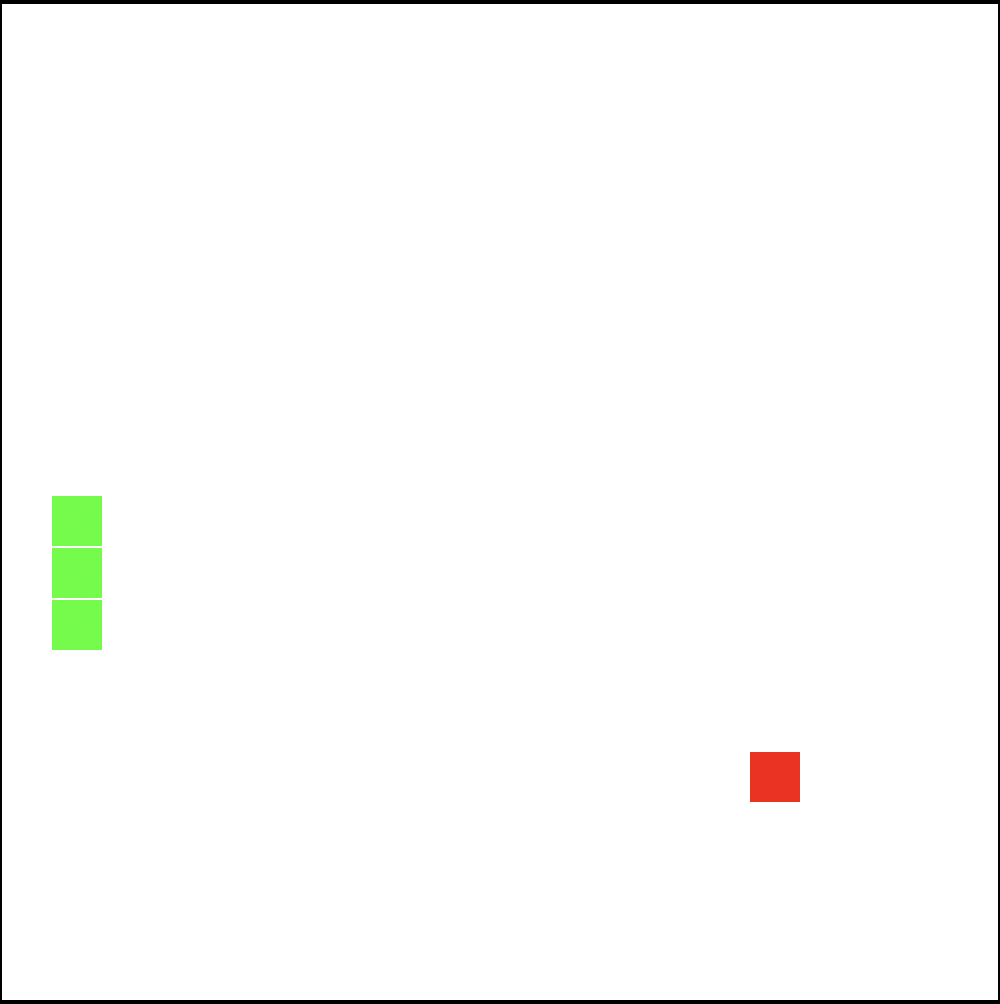
\includegraphics[width=5cm]{snake-game.png}
		\caption{First sketch of how the game should look like to the user}
	\end{figure}
	\section{Libraries}
	To implement our project we will mainly use 2htdp/image and 2htdp/universe.
	\section{Data types}
	To construct our appstate we thought to include these elements:
	\begin{itemize}
		\item a constant that represents the basic unit for the snake and the apple
		\item a data type that represents the snake
		\item a data type that represents the apple
		\item a data type that represents the available positions on the background
		\item a data type that represents whether the game has been lost or not
		\item a data type that represents whether the application has been quit or not
		\item (if we have time, we will implement something fo the points too)
	\end{itemize}
	
	In particular, the snake data type will be a structure and will preserve key informations about the snake itself, meaning that it will represent the length of the snake at a particular moment, the position of the head of the snake and the direction of the snake itself.
	We will create a basic unit for the snake that will be needed to render the snake on the background; in fact, the length of the snake will simply represent how many of these basic units will be needed to draw the snake. 
	
	We thought of the apple as simply being the position of the apple; this way, the draw function will draw the apple at he specified position and, if the head of the snake and the apple are at the same position, the position of the apple will be changed.
	
	To decide wether the game has been lost or not, we will use a simple boolean; when you are playing and the game hasn't been lost, this will be true, whilst loosing the game will change it to false. Clicking on the "r" button will make this again true if it was false, making the whole appstate back to its original state, starting a new game. 
	
	The "quit" will be just as the other type we described before, but in this case, this element will stop the loop, making the user stop the application.
	
	Here is the sketch of the design recipes needed for the data types mentioned before:
	\begin{itemize}
		\item a Snakeunit is an Image: (define SNAKEUNIT (rectangle 24 24 "solid" "green"))
		\item an Appleunit is an Image: (define APPLEUNIT (rectangle 24 24 "solid" "red"))
		\item a List$<$Posn$>$ is one of:\\
				- (cons Posn (cons Posn (cons Posn '())))\\
				- (cons Posn List$<$Posn$>$)
		\item AVAILABLEPOSITIONS is a List$<$Posn$>$ and it is a constant representing all the positions available on the background
		\item a Position is a member of the constant AVAILABLEPOSITIONS 
		\item a Snake is a struct:\\
				(make-snake position length direction)\\
				where:\\ 
				- position is a List<Position> (represents the positions of the snake-units)\\
				- length is a Number as such: the Number 3, length + 1 (represents the number of units that make up the snake at specified time)\\
				- direction is one of these String: "up", "left", "down", "right"  (represents the direction of the head of the snake)
		\item an Apple is a Posn (represents the randomic position of the apple at moment)
		\item a Game is a Boolean (\#true if the game is running; \#false if the game has been lost and it is currently on pause)
		\item a Quit is a Boolean (represents whether the application has been exit or not)
		\item an Appstate is a struct:\\
				(make-appstate snake apple game quit),\\
				where:\\
				- snake is a Snake\\
				- apple is an Apple\\
				- game is a Game\\
				- quit is a Quit
	\end{itemize}
	
	\section{About functions}
	To implement this game, we will use the big-bang function. In particular, we will need these core functionalities of the big-bang: 
	\begin{itemize}
		\item the on-draw
		\item the on-tick
		\item the on-key
		\item stop-when
	\end{itemize}
	
	For the on-draw, we will implement a draw function that will draw the whole appstate. This function will be divided in different auxiliary functions to first draw separately the different component of the game: we will implement a function to draw the snake based on the snake structure and a function to draw the apple. These two will be combined together to obtain the final result.
	
	The on-tick function will need instead two functions: one to change the position of the snake on-tick and the other one to change the rate of the clock as the game procedes. The rate of the clock needs to be increased whenever the snake eats a new apple.
	
	The on-key function will implement the functions to handle the keyboard; this function will need an auxiliary function to change the direction of the head of the snake.
	
	The stop-when will simply stop the game when the quit of the upstate will be changed to true.
	
	Here are some functions we thought about:
	\begin{itemize}
		\item draw-snake: Snake -$>$ Image (renders the snake)
		\item draw-apple: Apple -$>$ Image (renders the apple over the background)
		\item increment-dimension: Snake -$>$ Snake (Increments the dimensions of the snake if it eats the apple)
		\item update-snake-position: Snake -$>$ Snake (Updates the List<Posn> in the snake struct)
		\item increment-clock-rate: Snake Number -$>$ Number (Increments clock rate in relation to the dimensions of the snake)
		\item change-snake-direction: Snake -$>$ Snake (Changes snake direction)
		\item compute-apple-position: Apple -$>$ Apple (Chooses a position of the apple using the random function)
		\item update-apple-position: Apple -$>$ Apple (Changes apple position)
		\item draw-appstate: Appstate -$>$ Image (renders the whole appstate)
		\item handle-keyboard: Appstate -$>$ Appstate (Handles when keys are pressed)
		\item reset: Appstate -$>$ Appstate (Restarts the application)
		\item end-game: Appstate -$>$ Appstate (Escapes the application)
	\end{itemize}
\end{document}